\documentclass[11pt]{article}

\usepackage[letterpaper]{geometry}

\usepackage[utf8]{inputenc}
\usepackage{mathpazo}
\usepackage{amsmath}
\usepackage{amsfonts}
\usepackage{physics}
\usepackage{siunitx}

\usepackage{fancyhdr}

\usepackage{graphicx}
\usepackage{float}

\usepackage[shortlabels,inline]{enumitem}

% Hyperlinks with decent looking default colors.
\usepackage{hyperref}
\usepackage{xcolor}
\hypersetup{
  colorlinks,
  linkcolor={red!50!black},
  citecolor={blue!50!black},
  urlcolor={blue!80!black}
}

% For those sexy spaced low small caps from classic-thesis!
\usepackage{microtype}
\usepackage{textcase}
\DeclareRobustCommand{\spacedlowsmallcaps}[1]{%
  \textls[80]{\scshape\MakeTextLowercase{#1}}%
}

\pagestyle{fancy} 
\fancyhead{}
\rhead{Ali Ramadhan}
\lhead{12.818: Project one}
\chead{}
\cfoot{\thepage}
\renewcommand{\headrulewidth}{0pt}

\title{\spacedlowsmallcaps{\small 12.818: Introduction to Atmospheric Data and Large-scale Dynamics}\\ \spacedlowsmallcaps{\large Project two: Hydrostatic balance and the large-scale tilt of constant pressure surfaces}}
\author{Ali Ramadhan}
\date{\today}

% \renewcommand\thesection{\Alph{section}}

\begin{document}
\maketitle

In this project we will use the concept of hydrostatic balance to estimate the tilt, or rather the slope, of constant pressure surfaces in the atmosphere.

\section{Maps}
\begin{figure}
	\centering
	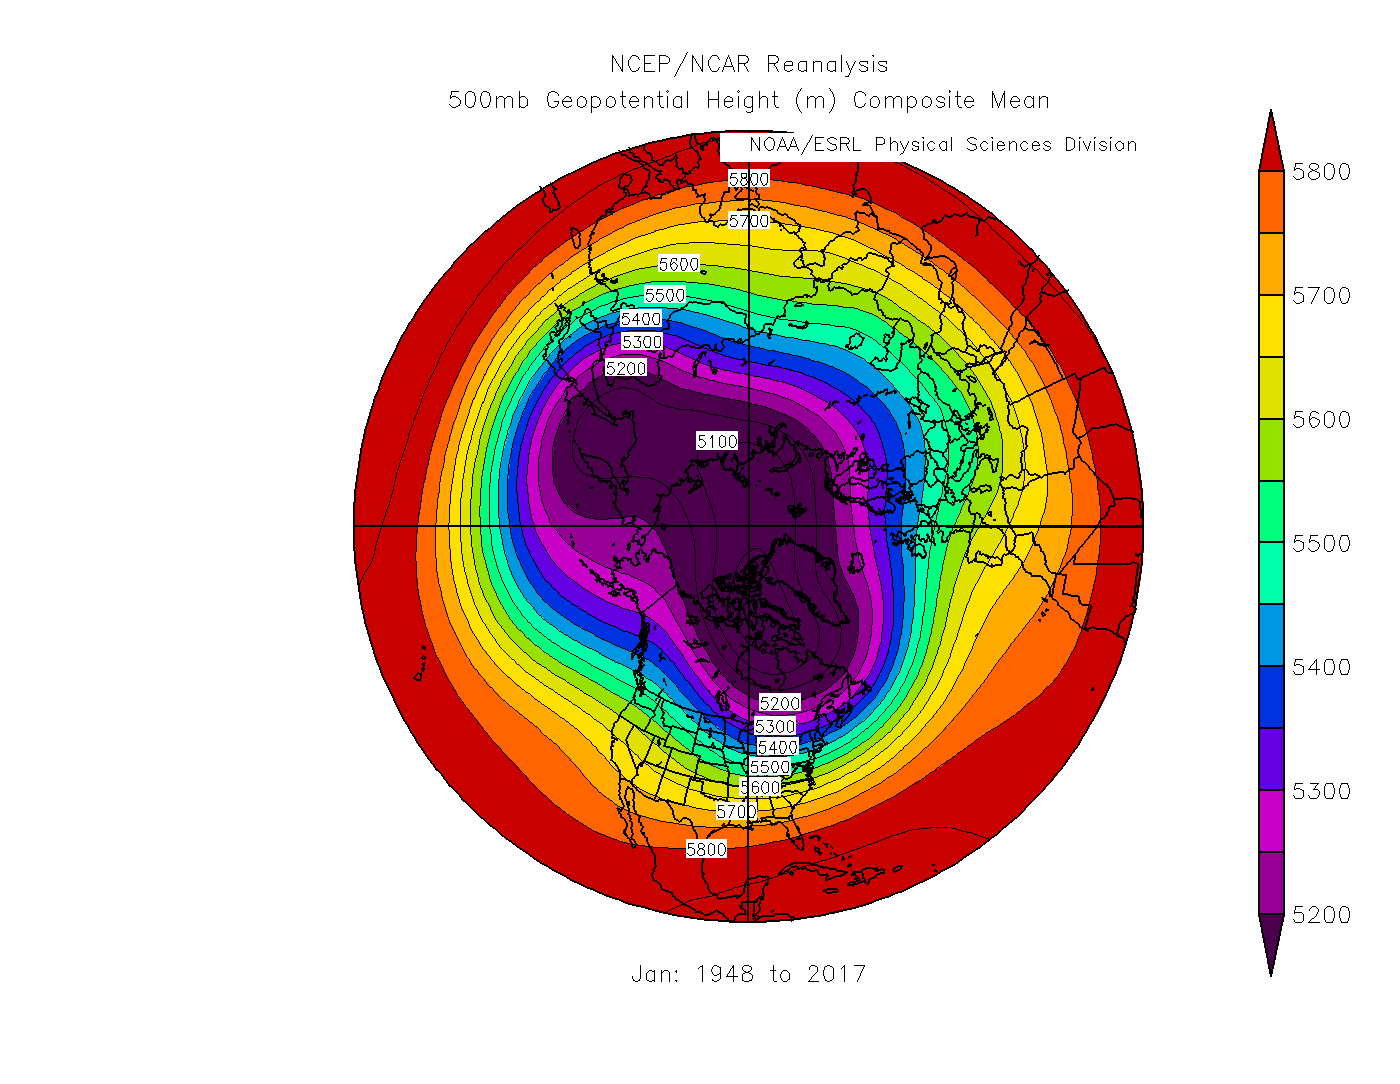
\includegraphics[width=\textwidth]{GeoHeight500hPa.png}
	\caption{The geopotential height of the \SI{500}{\hecto\Pa} constant pressure surface in meters (m) over the northern hemisphere in January. This plot was produced using NCEP reanalysis data averaged over the years 1948--2017.}
	\label{fig:GeoHeight500hPa}
\end{figure}

\section{Hydrostatic balance and the tilt of a constant pressure surface}

\section{Change of tilt with height}

\end{document}